
%!TEX TS-program = XeLaTeX
%!TEX TS-program = XeLaTeX
\documentclass[11pt]{article}

\usepackage{amssymb}
\usepackage{amsthm}
\usepackage{amsmath}
\usepackage{mathtools}

\usepackage{fancyhdr}
\usepackage{graphicx}
\usepackage[top=3cm, left=2cm, right=2cm, headheight = 90pt]{geometry}
\usepackage{xltxtra}
\usepackage[font=small,labelfont=bf]{caption}

\usepackage{multicol}

\renewcommand{\theenumi}{\alph{enumi}}


\def\leq{\leqslant}
\def\geq{\geqslant}
\def\N{\mathbb N}
\def\R{\mathbb R}
\def\Z{\mathbb Z}
\DeclarePairedDelimiter\set\{\}

\def\prob{}

\theoremstyle{definition}
\newtheorem{problem}{\prob}


\pagestyle{fancy}

%%!TEX TS-program = XeLaTeX

\fancyfoot[CE,CO]{}  % this is to remove page numbers (as you might want for single page docs)

%%!TEX TS-program = XeLaTeX
\renewcommand{\figurename}{Attēls}

\fancyhead[C]{{\Large\bf Strategies and tactics - Solutions}\\ \date}

\renewcommand{\theenumi}{\alph{enumi}}

\begin{document}
%\thispagestyle{fancy}
\noindent 
%\emph{\notes}

%1
\begin{problem}
\textit{[Bridge problem - "expanding a problem"]}

Why does this seem so hard? For some students the barrier of \textit{"this seems impossible"} actually becomes a self-fulfilling prophecy.

This problem is easy to crack just by using \textit{get your hands dirty} (aka \textit{work hard}) method - just systematically try out the possible options and soon you will hit the one that works, provided you do not give in to despair and give up.

This can also illustrate a more sophisticated  method - \textit{expanding} - in order to solve the problem. We try to pinpoint the exact difficult part of the problem, \textit{expand} it,  solve that expanded problem separately and then come back to the original problem.

Here, for example, the difficulty seems to be that two of the men are too slow... so we try to make it even worse - look at the same problem but with speeds $1$, $2$, $1000$, $1001$ and time limit of $1008$. In this expanded problem it is clear that two slower men have to cross over together and only once.  This easily leads to the fact that the two slowest can't be the first to cross (because there would be no way to get the lantern back) and they can't be the last to cross (because if the two slowest are alone on the near bank with lantern, then how did the lantern get there?).  Therefore the two slowest men cross on the second crossing. And indeed any remaining combination of people crossing on first and third crossings lead to a solution.

To apply it back to the original problem - 
\begin{itemize}
\item 1. and 2. cross over - $2$ minutes 
\item 1. crosses back - $1$ minute 
\item 5. and 10. cross over - $10$ minutes
\item 2. crosses back - $2$ minutes 
\item 1. and 2. cross over - $2$ minutes 
\end{itemize}
In total - $17$ minutes.
\end{problem}
%
\filbreak
%2
\begin{problem}
\textit{[9 dots - "thinking outside the box"]}

This problem has two \textit{outside the box} steps:
\begin{itemize}
\item Lines can be diagonal
\item Lines can literally go outside the box grid.
\end{itemize}

With these two steps and some work you can arrive at:
\begin{center}
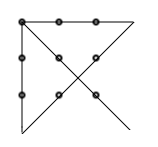
\includegraphics[width=2cm]{3by3Solved.png}
\captionof{figure}{3x3 dots solved}
\end{center}
\end{problem}
%

%3
\begin{problem}
\textit{[More dots - "reduction","thinking outside the box"]}
This is a visual example of reduction. 
\begin{enumerate}
\item $5 \times 5$ with $8$ lines  - imagine that middle $3 \times 3$ points are painted in green colour. \textit{Reducing} this problem to previous, we know how to connect those green points with $4$ lines. Remaining points are trivial since they are a rectangle (diagonal of the $9$ point solution nicely hits the corner of this rectangle)
\begin{center}
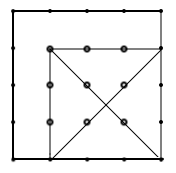
\includegraphics[width=2cm]{5by5Solved.png}
\captionof{figure}{5x5 dots solved}
\end{center}
\item $4 \times 4$ with $6$ lines - some people find this a bit more tricky (maybe because you have to go outside the "box" again), but it works exactly the same way
\begin{center}
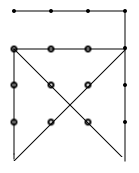
\includegraphics[width=2cm]{4by4Solved.png}
\captionof{figure}{4x4 dots solved}
\end{center}
\item $3 \times 4$ with $5$ lines - this is a very simple exercise in reduction, however usually people by now have fallen into a new kind of "box" and fail to notice the trivial solution
\begin{center}
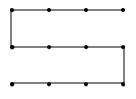
\includegraphics[width=2cm]{3by4Solved.png}
\captionof{figure}{3x4 dots trivial solution}
\end{center}
\item $4 \times 5$ with $7$ lines - this is really just an exercise in reduction (almost identical to $5 \times 5$)
\end{enumerate}
\end{problem}
%
\filbreak
%4
\begin{problem}
\textit{[Sultan's law - "symmetry"]}

The direct line of reasoning here leads into infinite sums and tricky probabilities. 

However an elegant argument via symmetry exists:
Assume $20$ years passed after the passing of law. Say, there have been in total $X$ births in this period. But the birth events are, unchangeably, $50/50$ chance events, so there will be $\frac{X}{2}$ boys born and $\frac{X}{2}$ girls born during this period!

Now, to the question of average size of the family. According to the new law, each family has exactly one boy.   We already proved, by symmetry, that there is equal amount of girls and boys, so, the average number of children in the family is $2$.

\end{problem}
%


%5
\begin{problem}
\textit{[Gambling problem - "symmetry"]}

This is an example that symmetry is strong, but sometimes tricky and un-intuitive.

\begin{enumerate}
\item "heads-heads-heads" vs "tails-tails-tails" - this is a fair game following an argument that if we just rename sides of the coin we can get one from another
\item "heads-heads-heads" vs "heads-heads-tails" - this is a fair game, because we can effectively ignore everything that happens before "heads-heads" event and then either of them wins with probability $\frac{1}{2}$ on the next toss
\item "tails-tails-heads" vs "heads-heads-tails" - this is a fair game, again, following the fact that you can get one from another by renaming sides of the coin
\item "tails-tails-heads" vs "heads-heads-heads" - this, however, is not a fair game (although "symmetry" kind of suggests it should be). How to see that? 

Well, the expected time, when we see "tails-tails" is the same as "heads-heads". 
But, if "heads-heads" happens, player, who betted on "heads-heads-heads" might still lose (if next toss is "tails"). 
However if the "tails-tails" happens, the player who betted on "tails-tails-heads" can not loose anymore (there is no way to go from "tails-tails" to "heads-heads-heads" without going through "tails-tails-heads"
\end{enumerate}

Here is a VSouce2 video about this problem: \url{https://www.youtube.com/watch?v=s4tyO4V2im8&list=PLVQ8GqrsK7VDLX9Zau9bN7BiT-GIHpwGT&index=10}
\end{problem}
%
\end{document}
